\chapter{双波干涉}\label{ch:b2:two-wave-interference}

肥皂泡由无色液体构成，却闪烁着
色彩；湿路面上的油膜呈现同样的彩虹色带；蜻蜓的
翅膀闪着绿色与紫色的光。这些颜色都不是
源于色素，而是同一束光波的两个副本，
在薄膜的两个表面分别反射，经过一段延迟后到达，并
相互加强或相互抵消——这就是两列波的\emph{干涉}
现象。杨于 1801 年以此证明光是一种波，
装置为两条狭缝与一支蜡烛；本章给出公式、
杨氏条纹的几何，以及条纹得以存续的两个条件——时间
相干性与空间相干性，以及薄膜干涉的
颜色。

\begin{omfigure}
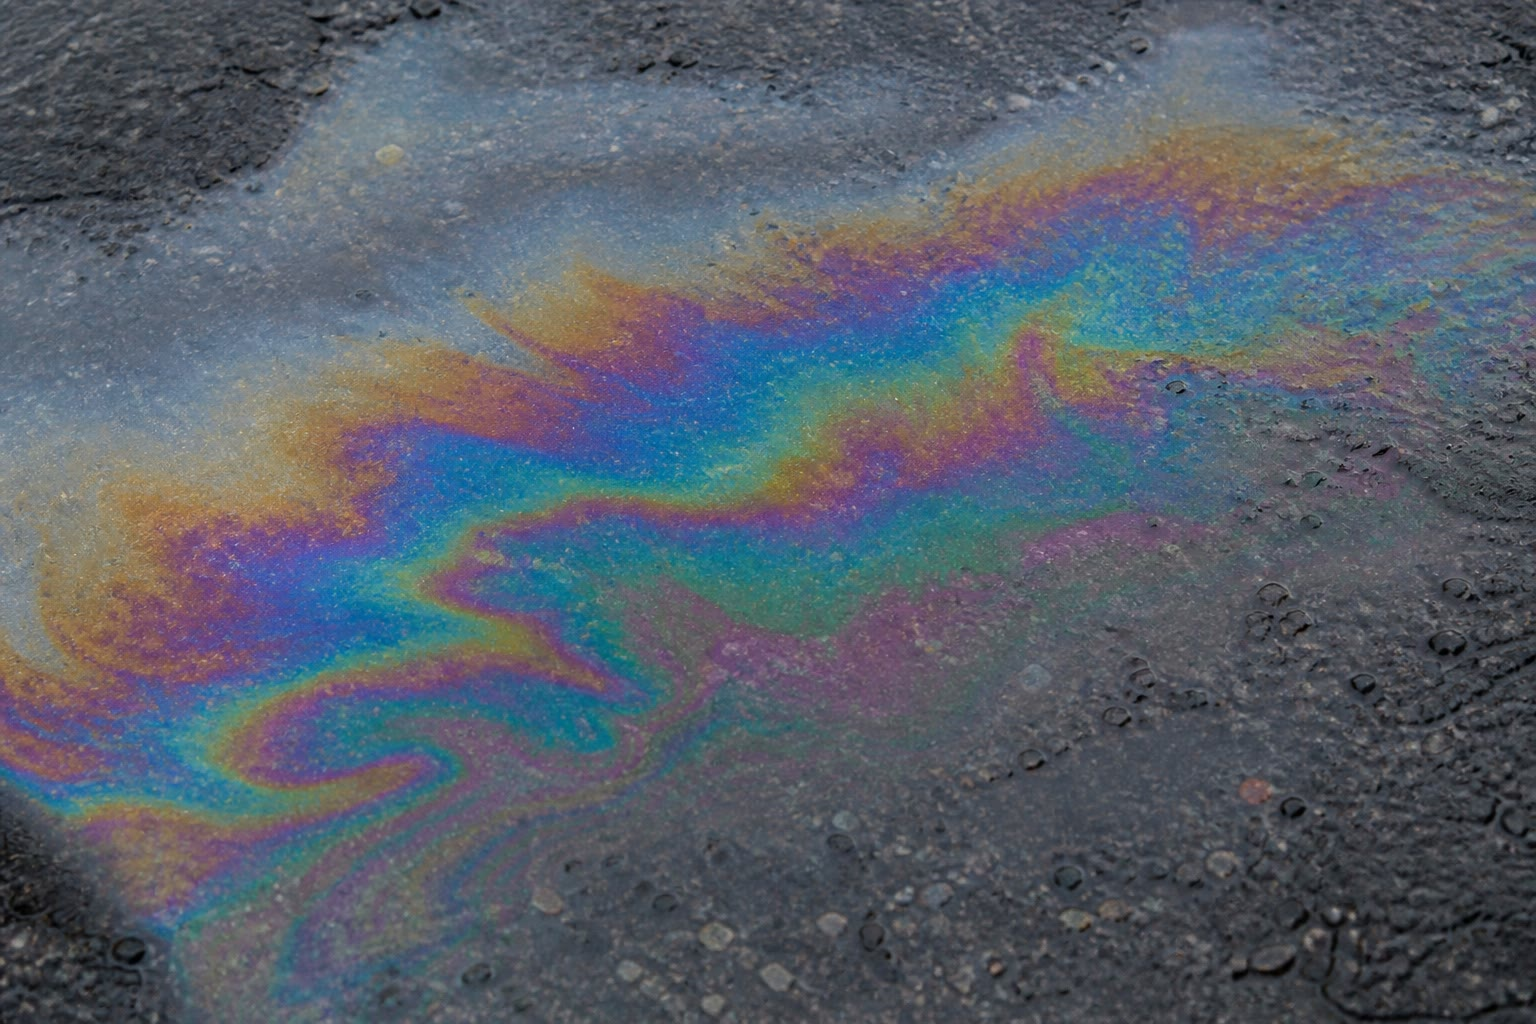
\includegraphics[width=0.58\linewidth]{images/book4/ai/b4-19-oil-film-puddle.jpg}

{\small 湿路面上的油膜：两束反射光分别来自两个表面，膜厚随位置而变化——凡 $2ne$ 取值合适之处，颜色都明亮。}
\end{omfigure}


\section{干涉公式}

\begin{theorem}[双波干涉]\label{thm:b2:two-wave-interference:formula}
\index{干涉}\index{光程差}\index{干涉级次}\index{对比度（条纹）}
两束强度分别为 $I_1$、$I_2$ 的相干单色波，
其相位差 $\Delta\varphi$ 在点 $M$ 处产生的强度为
\[
I(M) = I_1 + I_2 + 2\sqrt{I_1I_2}\,\cos\Delta\varphi(M) , \qquad
\Delta\varphi = \frac{2\pi}{\lambda_0}\,\delta(M) ,
\]
其中 $\delta$ 为从光源到 $M$ 的两条路径之间的\emph{光程差}，
强度取极大值（$I_1 + I_2 +
2\sqrt{I_1I_2}$）处，其中 $\delta = p\lambda_0$，$p$ 为整数，
称为\emph{干涉级次}。极小值为（$I_1 + I_2 - 2\sqrt{I_1I_2}$），此时 $\delta = (p +
\tfrac12)\lambda_0$。条纹的\emph{对比度}（可见度）为
\[
V = \frac{I_{\max} - I_{\min}}{I_{\max} + I_{\min}} = \frac{2\sqrt{I_1I_2}}{I_1 + I_2} ,
\]
两强度相等时对比度等于 $1$，此时极小处完全变暗：
$I = 2I_0(1 + \cos\Delta\varphi) = 4I_0\cos^2(\Delta\varphi/2)$。
\end{theorem}

\begin{proof}
$s = a_1\cos(\omega t - \varphi_1) + a_2\cos(\omega t - \varphi_2)$；$\langle s^2\rangle$ 的求法同
\cref{ch:b2:scalar-light-model}，其中 $\Delta\varphi$ 在探测期间保持不变；
$I_i = \tfrac12Ka_i^2$。两列同时自光源出发的波，
经光程 $L_1$、$L_2$ 传播后，其相位差为
$2\pi(L_2 - L_1)/\lambda_0$（每次使相位符号反转的反射再附加 $\pi$，
见\cref{ch:b2:wave-interfaces}）。
\end{proof}

\begin{remark}[三个条件]\label{rem:b2:two-wave-interference:conditions}
\index{相干性（空间）}\index{相干性（时间）}
条纹只有在以下条件下才存在：（1）两列波来自\emph{同一
光源}（同一振动的两个副本，否则 $\Delta\varphi$ 是随机的）；（2）
光程差小于相干长度，$|\delta| < \ell_c$
（\emph{时间相干性}：超出此范围时，两个副本属于不同的
波列）；（3）光源足够小，使其不同点
不会产生彼此错位而相互抹去的条纹系统
（\emph{空间相干性}，见下文）。第四个条件通常也满足：
两列波不得具有相互垂直的偏振态（否则二者
按强度相加，如同两支火把）。
\end{remark}

\section{杨氏双缝}

\begin{proposition}[波前分割：杨氏实验]\label{prop:b2:two-wave-interference:young}
\index{杨氏双缝}\index{条纹间距}\index{波前分割}
点光源 $S$（或一条狭缝）照亮两条窄而平行的狭缝
$S_1$、$S_2$ 相距 $a$，且与 $S$ 等距；屏幕位于
距离 $D \gg a$ 处。屏上高度为 $x$（平行于
$a$ 方向）处的光程差为
\[
\delta = S_2M - S_1M \approx \frac{ax}D ,
\]
屏上为直的等间距条纹，亮纹位于 $x_p =
p\lambda D/a$ 处，\emph{条纹间距}为
\[
i = \frac{\lambda D}a .
\]
条纹在双缝之后处处存在（它们\emph{并非
定域}）；若在双缝后放置焦距为 $f$ 的透镜，则
条纹可在其焦平面上观察到，此时 $i = \lambda f/a$（“无穷远”条纹）。
强度为 $4I_0\cos^2(\pi ax/\lambda D)$。
\end{proposition}

\begin{proof}
$S_2M^2 - S_1M^2 = [(x + a/2)^2 - (x - a/2)^2] = 2ax$，且 $S_2M + S_1M \approx 2D$，
于是 $\delta \approx 2ax/2D$。两相邻级次相差 $\lambda$，即 $\Delta x = \lambda D/a$。
若加入透镜，则从两狭缝以与光轴成 $\theta$
角射出的两列波光程差为 $a\sin\theta \approx a\theta$，并在 $x = f\theta$ 处会合。
\end{proof}

\begin{omfigure}
\begin{tikzpicture}[font=\small, x=1cm, y=1cm, >=Stealth]
  \begin{scope}
    \fill (-3.6,0) circle (1.5pt); \node[font=\footnotesize] at (-3.8,0.3) {$S$};
    \draw[thick] (-1.5,-1.6) -- (-1.5,-0.35) (-1.5,-0.15) -- (-1.5,0.15) (-1.5,0.35) -- (-1.5,1.6);
    \fill (-1.5,0.25) circle (1.2pt) node[left, font=\footnotesize] {$S_1$}; \fill (-1.5,-0.25) circle (1.2pt) node[left, font=\footnotesize] {$S_2$};
    \draw[<->] (-1.1,0.25) -- (-1.1,-0.25) node[midway, right, font=\footnotesize] {$a$};
    \draw[thick] (2.8,-1.8) -- (2.8,1.8);
    \fill (2.8,0.9) circle (1.5pt) node[right, font=\footnotesize] {$M$, $x$};
    \draw[omDef, thick] (-1.5,0.25) -- (2.8,0.9); \draw[omDef, thick] (-1.5,-0.25) -- (2.8,0.9);
    \draw[omDef, thick] (-3.6,0) -- (-1.5,0.25); \draw[omDef, thick] (-3.6,0) -- (-1.5,-0.25);
    \draw[<->] (-1.5,-2.0) -- (2.8,-2.0) node[midway, below, font=\footnotesize] {$D$};
    \node[font=\footnotesize] at (0.6,-1.5) {$\delta \approx ax/D$};
    % fringes on the screen
    \foreach \y in {-1.5,-1.0,-0.5,0,0.5,1.0,1.5} \fill[omThm!50] (2.85,{\y-0.12}) rectangle (3.15,{\y+0.12});
    \draw[<->] (3.35,0) -- (3.35,0.5) node[midway, right, font=\footnotesize] {$i$};
  \end{scope}
  \begin{scope}[xshift=9.3cm]
    \begin{axis}[omaxis, axis x line=bottom, axis y line=left, width=4.2cm, height=4.0cm, at={(0,-1.7cm)},
        xlabel={$x/i$}, ylabel={$I/I_0$}, xmin=-2.5, xmax=2.5, ymin=0, ymax=4.4, xtick={-2,-1,0,1,2}, ytick={2,4}, samples=200,
        xlabel style={at={(axis description cs:0.5,-0.14)}, anchor=north},
        ylabel style={at={(axis description cs:-0.12,0.5)}, rotate=90, anchor=south}]
      \addplot[omDef, thick, domain=-2.5:2.5] {4*cos(deg(pi*x))^2};
      \addplot[omThm, thick, dashed, domain=-2.5:2.5] {2+1.2*cos(deg(2*pi*x))};
    \end{axis}
  \end{scope}
\end{tikzpicture}

{\small 左：杨氏双缝——同一光源发出的波的两个副本在屏上相遇，
光程差为 $ax/D$；亮条纹间距为
$\lambda D/a$。右：光强分布 $4I_0\cos^2(\pi x/i)$，对应等幅波
（实线）及对比度降低的情形（虚线）。}
\end{omfigure}

\begin{example}[数值，以及白光]\label{ex:b2:two-wave-interference:numbers}
$a = \qty{0.5}{mm}$，$D = \qty{2}{m}$，$\lambda = \qty{600}{nm}$，则 $i = \qty{2.4}{mm}$——
条纹足够大，足以看清，这正是杨氏双缝须靠近、屏须
远的原因。用白光时，每种颜色各自形成条纹，全部
在中心重合（$\delta = 0$）：中央为白色亮纹，随后
因级次逐渐错开而出现彩色条纹（红光的 $i$ 为
紫光的 $1.8$ 倍），若干级次之后呈现均匀的泛白场——
白光的相干长度约为一微米，相当于两三个
波长。用分光计对准那“白色”场时，仍能看到
在使 $\delta = (p + \tfrac12)\lambda$ 成立的波长处呈现暗带：一种
\emph{沟纹光谱}。
\end{example}

\begin{proposition}[空间相干性：光源须很小]\label{prop:b2:two-wave-interference:spatial}
\index{空间相干性}\index{扩展光源}
扩展光源的每一点各自产生一组干涉条纹；一个
在狭缝前方、横向位移为 $b$、距离为 $L$ 处的光源点，使
条纹平移 $x = bD/L$（光程差增加
$ab/L$）。宽度为 $b$ 的光源使条纹铺开一个条纹间距，
则对比度消失，条件为
\[
\frac{ab}L \approx \lambda , \qquad\text{即狭缝对光源所张角度满足 } \frac bL \gtrsim \frac\lambda a .
\]
两条狭缝必须位于光的\emph{相干面积}之内——
即光源发出的波具有确定
相位的区域，宽度为 $\lambda L/b$。太阳光（$b/L = \qty{0.5}{\degree} = \qty{9}{mrad}$）
给出相干宽度 $\lambda/0.009 \approx \qty{60}{\micro m}$：杨氏需用一个
针孔来拓宽它。
\end{proposition}

\begin{proof}
对高度为 $b$ 的光源点，附加光程 $SS_2 - SS_1 \approx -ab/L$
与 $ax/D$ 相加，图样平移 $x = bD/L$。将
错位的 $\cos^2$ 图样沿宽度为 $b$ 的光源积分，得到对比度
$|\operatorname{sinc}(\pi ab/\lambda L)|$，在 $ab/L = \lambda$ 时为零。
\end{proof}

\begin{omfigure}
\begin{tikzpicture}[font=\small, x=1cm, y=1cm, >=Stealth]
  \draw[thick, omThm] (-4.2,-0.4) -- (-4.2,0.4); \node[omThm, font=\footnotesize] at (-4.6,0) {$b$};
  \draw[thick] (-1.0,-1.5) -- (-1.0,-0.3) (-1.0,-0.1) -- (-1.0,0.1) (-1.0,0.3) -- (-1.0,1.5);
  \draw[omDef] (-4.2,0.4) -- (-1.0,0.2); \draw[omDef] (-4.2,0.4) -- (-1.0,-0.2);
  \draw[omProp] (-4.2,-0.4) -- (-1.0,0.2); \draw[omProp] (-4.2,-0.4) -- (-1.0,-0.2);
  \draw[<->] (-4.2,-1.9) -- (-1.0,-1.9) node[midway, below, font=\footnotesize] {$L$};
  \draw[thick] (3.0,-1.8) -- (3.0,1.8);
  \foreach \y in {-1.5,-1.0,-0.5,0,0.5,1.0,1.5} \fill[omDef!50] (3.05,{\y-0.1}) rectangle (3.3,{\y+0.1});
  \foreach \y in {-1.5,-1.0,-0.5,0,0.5,1.0,1.5} \fill[omProp!50] (3.35,{\y-0.1+0.25}) rectangle (3.6,{\y+0.1+0.25});
  \node[font=\footnotesize] at (-0.5,2.2) {每个光源点：各自的条纹，平移 $bD/L$};
  \node[font=\footnotesize] at (-0.5,-2.5) {$ab/L \approx \lambda$ 时对比度消失};
\end{tikzpicture}

{\small 空间相干性：扩展光源的上、下两端
发出的条纹系统彼此错开；当错开量
达到一个条纹间距时，图样被抹平。}
\end{omfigure}

\section{薄膜：分振幅干涉}

\begin{proposition}[薄膜干涉]\label{prop:b2:two-wave-interference:film}
\index{薄膜干涉}\index{分振幅}\index{等倾条纹}\index{等厚条纹}
空气中、折射率为 $n$、厚度为 $e$ 的薄膜，以入射角 $i$ 照明，
（折射角为 $r$），在其两个表面反射出两束波，
其光程差为
\[
\delta = 2ne\cos r \ (+\tfrac{\lambda_0}2) ,
\]
附加的半个波长来自反射时的符号反转，
即在第一面（光密介质上的反射）发生，在第二面不发生，
（见\cref{ch:b2:wave-interfaces}）。亮纹位于 $2ne\cos r =
(p + \tfrac12)\lambda_0$，暗纹位于 $2ne\cos r = p\lambda_0$ 处——厚度趋于零的
薄膜\emph{不反射任何光}（排液中肥皂
膜的黑色顶部）。对厚度均匀的薄膜，条纹仅依赖于 $i$，
并在无穷远处观察（\emph{等倾}条纹）；对
厚度缓变的楔形薄膜，在近正入射下，它们
沿等 $e$ 线分布，定域于薄膜上
（\emph{等厚}条纹）：夹角为 $\alpha$ 的空气劈尖呈现
间距为 $\lambda_0/2\alpha$ 的直条纹；半径为 $R$ 的透镜置于平板上，给出
\emph{牛顿环}，暗环半径为 $r_p = \sqrt{p\lambda_0R}$。
\end{proposition}

\begin{proof}
几何关系：在第一面折射的波两次穿过薄膜，
（在玻璃中走过 $2e/\cos r$，光程为 $2ne/\cos r$），而在第一面反射的波
在空气中前进 $2e\tan r\sin i$；两者之差为
$2ne/\cos r - 2e\tan r\sin i = 2ne\cos r$，其中 $\sin i = n\sin r$。对于
楔形，$e = \alpha x$，相邻暗条纹位于 $2\alpha x = p\lambda$；对于
透镜，$e \approx r^2/2R$。
\end{proof}

\begin{omfigure}
\begin{tikzpicture}[font=\small, x=1cm, y=1cm, >=Stealth]
  \begin{scope}
    \fill[omDef!15] (-3,-0.9) rectangle (3,0.9); \draw[thick] (-3,0.9) -- (3,0.9) (-3,-0.9) -- (3,-0.9);
    \node[font=\footnotesize] at (2.4,0) {$n$}; \draw[<->] (-2.7,-0.9) -- (-2.7,0.9) node[midway, left, font=\footnotesize] {$e$};
    \draw[omThm, thick, ->] (-2.2,2.2) -- (-0.9,0.95);
    \draw[omThm, thick, ->] (-0.85,0.92) -- (0.4,2.2);
    \draw[omProp, thick] (-0.9,0.9) -- (-0.2,-0.9) -- (0.5,0.9);
    \draw[omProp, thick, ->] (0.5,0.92) -- (1.75,2.2);
    \node[font=\footnotesize] at (-1.7,1.85) {$i$}; \node[font=\footnotesize] at (-0.75,-0.0) {$r$};
    \node[font=\footnotesize] at (0,-1.4) {$\delta = 2ne\cos r$ (+ $\lambda/2$)};
  \end{scope}
  \begin{scope}[xshift=7.8cm]
    \draw[thick] (-2.6,0) -- (2.6,0);
    \draw[thick] (-2.6,0.05) arc[start angle=-90, end angle=-60, radius=14] ;
    \draw[thick] (-2.6,0.05) -- (2.6,0.55);
    \foreach \x in {-2.0,-1.3,-0.6,0.1,0.8,1.5,2.2} \draw[omThm, very thick] (\x,-0.25) -- (\x,-0.45);
    \node[font=\footnotesize] at (0,-0.85) {空气劈尖：每隔 $\lambda/2\alpha$ 一条暗纹};
    \draw[omDef, thick] (-2.6,0.05) -- (-2.6,0); \node[font=\footnotesize] at (2.9,0.3) {$\alpha$};
  \end{scope}
\end{tikzpicture}

{\small 左：薄膜的两束反射光——每个表面各一束，
第二束因往返穿过薄膜而延迟。右：两块平板间的空气劈尖
显示等厚的直条纹，
间隙每增加半个波长，便多出一条。}
\end{omfigure}

\begin{example}[肥皂、油膜与蜻蜓]\label{ex:b2:two-wave-interference:colours}
一层厚 \qty{300}{nm} 的肥皂膜（$n = 1.33$），垂直入射观察：
亮纹条件为 $2ne = (p + \tfrac12)\lambda$，即 $\lambda = 798/(p + \tfrac12)$ nm：\qty{532}{nm}
（绿色，$p = 1$）落在可见光范围内，\qty{400}{nm} 处为暗带；
薄膜呈绿色。随液膜排出而变薄，颜色依次
经历一系列变化，最终呈黑色。一层油膜（\qty{400}{nm}，$n = 1.45$）漂浮在
水面（$1.33$）上：第二次反射朝向较低折射率一侧，不发生半波损失，
故仍有 $\delta = 2ne + \lambda/2$，亮纹条件为 $2ne =
(p + \tfrac12)\lambda$：\qty{464}{nm}（$p = 2$），呈蓝色。蝴蝶翅膀的虹彩、
甲虫外壳的虹彩与光盘的彩色都属同一类干涉，
（光盘的情形涉及多束波，见\cref{ch:b2:gratings}），
因而它们随角度变化——$\delta$ 依赖于 $\cos r$——
而颜料的颜色则不随角度改变。
\end{example}

\begin{method}[求解干涉问题]\label{met:b2:two-wave-interference:method}
(1) 确定从光源到 $M$ 的两条路径，并计算
光程差 $\delta(M)$，对每次
发生半波损失的反射附加 $\lambda/2$。(2) $I = I_1 + I_2 + 2\sqrt{I_1I_2}\cos(2\pi\delta/\lambda)$；
亮纹位于 $\delta = p\lambda$。(3) 条纹间距由 $\delta(M + \Delta M) - \delta(M) =
\lambda$ 给出。(4) 检验时间相干性（$\delta_{\max} < \ell_c$，
可见条纹数 $\sim\lambda/\Delta\lambda$）及空间相干性（光源张角
$< \lambda/a$）。(5) 说明条纹定域的位置（两个
点光源时处处可见；等厚条纹在膜上；
等倾条纹则在无穷远处）。
\end{method}

\section{练习}

\begin{exercise}[$\star$]\label{exo:b2:two-wave-interference:1}
杨氏双缝间距 $a = \qty{0.40}{mm}$，屏幕距离 $D = \qty{1.5}{m}$，$\lambda =
\qty{633}{nm}$：条纹间距；位于 $x = \qty{1.0}{cm}$ 处的条纹级次；
第十条暗纹的位置；双缝间距改为 \qty{2}{mm} 时的条纹间距，
以及置于水中（$n = 1.33$）时的条纹间距。
\end{exercise}

\begin{exercise}[$\star$]\label{exo:b2:two-wave-interference:2}
两列强度分别为 $I_0$ 与 $I_0/4$ 的波发生干涉：求 $I_{\max}$、$I_{\min}$，
对比度。对 $I_0$ 与 $I_0/100$ 亦求同样的量：为何
两束光强相差如此悬殊时条纹仍可见？杨氏双缝中的一条缝被一块
透过率为 $50\%$ 的灰色滤光片遮住，求新的对比度。
\end{exercise}

\begin{exercise}[$\star$]\label{exo:b2:two-wave-interference:3}
一层厚 \qty{250}{nm}（$n = 1.33$）的肥皂膜，垂直入射观察：
求可见光中反射最强和最弱的波长，并说明其颜色。另一
厚 \qty{1.0}{\micro m} 的薄膜中，可见光范围内有几个亮纹波长，
人眼看到的是什么颜色？
\end{exercise}

\begin{exercise}[$\star$]\label{exo:b2:two-wave-interference:4}
半径为 $R = \qty{2.0}{m}$ 的透镜与平板之间的牛顿环，在钠光下：
求前三个暗环的半径；
半径 \qty{1}{cm} 之内的环数；中心是亮还是暗，为什么？
若间隙充满水，结果有何变化？
\end{exercise}

\begin{exercise}[$\star\star$]\label{exo:b2:two-wave-interference:5}
\emph{白光。}杨氏双缝用白光（$400$--\qty{700}{nm}）照明，
$a = \qty{0.5}{mm}$，$D = \qty{1}{m}$。(a) 紫光与红光的条纹间距；
红光的第二级、紫光的第三级亮纹位置。(b)
从第几级开始，相邻各级的红光与紫光条纹
开始重叠？(c) 在 $x = \qty{5}{mm}$ 处，哪些波长缺失
（沟纹光谱）？(d) 解释从中心向外看到的颜色
顺序。
\end{exercise}

\begin{exercise}[$\star\star$]\label{exo:b2:two-wave-interference:6}
\emph{光源尺寸。}钠灯经光源狭缝照明杨氏双缝（$a = \qty{1.0}{mm}$），
光源狭缝位于 $L = \qty{40}{cm}$ 处。(a) 为保证较好的对比度，光源狭缝的最大宽度
（取 $ab/L < \lambda/4$）。(b) 光源狭缝
加宽至 \qty{0.5}{mm}，求对比度（使用 $|\operatorname{sinc}(\pi ab/\lambda L)|$）。
(c) 为何不能直接用裸灯（宽 \qty{1}{cm}）？(d) 以太阳为光源，
其张角为 \qty{9}{mrad}：能产生条纹的
双缝最大间距为多少？
\end{exercise}

\begin{exercise}[$\star\star$]\label{exo:b2:two-wave-interference:7}
\emph{劳埃德镜。}点光源距平面镜高 $h = \qty{0.2}{mm}$，
屏幕距离 $D = \qty{1.0}{m}$，$\lambda = \qty{500}{nm}$：直射波
与经平面镜反射的波发生干涉（虚光源位于
$-h$ 处）。(a) 条纹间距。(b) 镜面边缘（$x = 0$）处的条纹为暗纹，
这说明了关于反射的什么？(c) 若光源相干长度为
\qty{50}{\micro m}，可见条纹数为多少？(d) 为何这种装置可作为
射电天文学家观测升起恒星的
“海面干涉仪”？
\end{exercise}

\begin{exercise}[$\star\star$]\label{exo:b2:two-wave-interference:8}
\emph{空气劈尖。}两块长 \qty{10}{cm} 的玻璃板一端接触，
另一端由直径为 $d$ 的细丝隔开；用钠光照明时数得
$42$ 条暗纹。(a) 求 $d$。(b) 条纹间距。(c) 若间隙充满水，
条纹数是多少？(d) 若将两板远端略微压紧，
条纹将如何变化？计数四分之一条纹，
能给出 $d$ 的何种精度？
\end{exercise}

\begin{exercise}[$\star\star$]\label{exo:b2:two-wave-interference:9}
\emph{水面油膜。}一层油膜（$n = 1.45$），厚度为 $e$，漂浮于水面
（$n = 1.33$）上。(a) 两次反射中哪一次发生半波损失？求光程差。
(b) 当 $e = \qty{400}{nm}$ 垂直入射时：
求加强与相消的反射波长，并说明颜色。(c) 能呈紫色的
最薄膜厚度（\qty{420}{nm}）。(d) 为何斜看时颜色向
蓝色方向偏移？(e) 对于折射率
\emph{介于}两种介质之间的薄膜（如玻璃上的镀膜），
结果有何变化？
\end{exercise}

\begin{exercise}[$\star\star\star$]\label{exo:b2:two-wave-interference:10}
\emph{单缝上的玻片。}厚度为 $e = \qty{20}{\micro m}$
，折射率为 $1.5$ 的玻璃片覆盖杨氏双缝的缝 $S_1$（$a = \qty{1}{mm}$，$D =
\qty{2}{m}$，$\lambda = \qty{500}{nm}$）。(a) 求附加光程；条纹移动了多少条
并向哪个方向移动？(b) 用白光照明时，
（现已移位的）白光中央条纹去往何处——它是否
仍可见？相干长度为 \qty{1.5}{\micro m}。(c) 如何利用白光
图样测量 $e$？(d) 将玻璃片倾斜后，移动量随之增大——
试证明一阶近似下其增长量为 $e(n - 1)\theta^2/2 \times (1 + 1/n)$，
并估算 \qty{5}{\degree} 时的移动量。
\end{exercise}

\begin{exercise}[$\star\star\star$]\label{exo:b2:two-wave-interference:11}
\emph{恒星干涉仪。}两面相距 $a$ 的镜子
收集恒星的光并使其发生干涉。恒星可视为
角直径为 $\theta$ 的均匀圆盘，圆盘上的每一点都使条纹移动，
且当 $a = 1.22\lambda/\theta$ 时对比度消失（在本阶段不加证明地承认，
即圆盘情形下的 $ab/L = \lambda$）。(a) 参宿四，$\theta = \qty{0.047}{''}$
（角秒），$\lambda = \qty{570}{nm}$：使条纹
消失的基线长度（迈克耳孙，1920 年，威尔逊山）。(b) 为何单台
口径为 \qty{2.5}{m} 的望远镜不能分辨该圆盘（其极限为 $1.22\lambda/d$）？
(c) 现代干涉仪把相距 \qty{100}{m} 的望远镜连接起来，可测的最小
直径。(d) 为何两路光程须在相干长度之内相等，
对于 \qty{10}{nm} 滤光片，该长度是多少？
\end{exercise}

\begin{exercise}[$\star\star\star$]\label{exo:b2:two-wave-interference:12}
\emph{等倾干涉环。}厚度为 $e =
\qty{2.0}{mm}$，折射率为 $1.5$，由宽钠光源照明；反射光
经焦距为 $f = \qty{50}{cm}$ 的透镜聚焦。(a) 试证明：
干涉环位于角度 $i_p$ 处，满足 $2ne\cos r_p = (p + \tfrac12)\lambda$（亮纹）；
且在中心附近 $\cos r \approx 1 - i^2/2n^2$。(b) 中心处的
级次是多少？中心是否为亮纹？(c) 焦平面上前三个亮环的
半径。(d) 为何这些环在扩展光源下可见，
而杨氏条纹需要窄光源？（定域于
无穷远。）
\end{exercise}

\begin{omfigure}
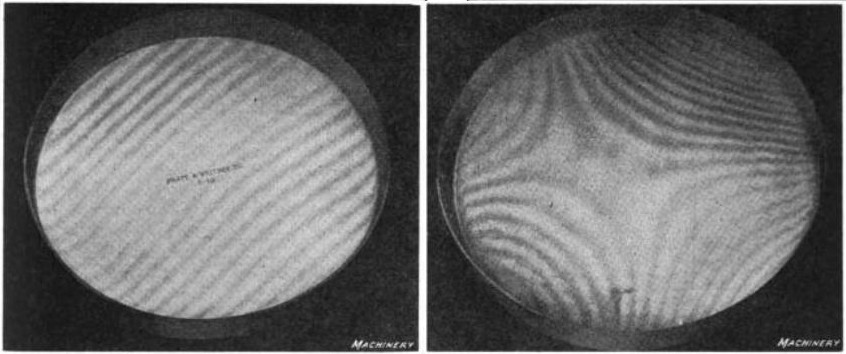
\includegraphics[width=0.62\linewidth]{images/book4/optical-flat-fringes.jpg}

{\small 约 1915 年一张机械师的照片：光学平晶与待检钢面之间的等厚条纹，平面处为直条纹，磨损处为弯曲条纹——每一条纹对应半个波长的台阶。}
\end{omfigure}

\section{问题：菲涅耳镜与油膜}

\begin{problem}[{周末问题——1816 年的干涉仪，以及水洼上的
彩虹：一束波的两种分割方式，以及限制两者的两种
相干性}]
\label{pb:b2:two-wave-interference:1}

\medskip
\noindent\textbf{第一部分——菲涅耳镜。}
两面平面镜沿一条直线相接，夹角 $\alpha =
\qty{5.0e-3}{rad}$；狭缝光源 $S$ 与该直线平行，距其 $d =
\qty{20}{cm}$，屏幕在其后 $D = \qty{1.5}{m}$ 处。$\lambda =
\qty{589}{nm}$（钠）。
\begin{enumerate}
  \item 证明两面镜子给出两个虚像 $S_1$、$S_2$，它们是
        $S$ 的像，位于以接缝线为中心、半径为 $d$ 的圆上，
        两者相距 $a = 2\alpha d$，并求其数值。
  \item 为何来自 $S_1$ 与 $S_2$ 的波会干涉，
        而两盏独立灯所发出的波却不会？
  \item 屏上的条纹间距（光源到屏幕的距离
        $\approx d + D$）；横跨两束反射光重叠的
        宽 \qty{5}{mm} 区域的条纹数。
  \item 该区域边缘处的干涉级次，
        是否低于灯的相干长度（\qty{2}{cm}）所限定的界限？
  \item 光源狭缝宽 \qty{20}{\micro m}：其两条边缘所产生的
        条纹移动量（每个光源点都成像为两个虚点，
        条纹系统移动 $bD'/d$，其中 $D' =
        d + D$）；对比度是否保持（与 $i$ 相比）？
  \item 狭缝加宽至 \qty{0.1}{mm}：对比度，用
        $|\operatorname{sinc}(\pi ab/\lambda d)|$ 计算。
  \item 两面镜子分别反射 $90\%$ 与 $80\%$ 的光：条纹的
        对比度。
  \item 将一块厚 \qty{10}{\micro m}（$n = 1.5$）的玻璃片
        置于一面镜子前：图样的移动量（以条纹计）；能否用钠光
        追踪？白光又如何？
  \item 将钠灯换成白光：描述屏幕上的图样；
        中央两侧各有多少条彩色条纹？
\end{enumerate}

\medskip
\noindent\textbf{第二部分——油膜。}
一层油膜（$n = 1.45$）覆盖在湿润路面（$n_{\text{水}} = 1.33$）上，
在阴天天光照射下，并以接近垂直入射的方向观察。
\begin{enumerate}[resume]
  \item 两个界面上的反射哪一次会反转符号？光程差
        及呈亮色的条件。
  \item 呈红色的最薄区域的厚度（$\lambda =
        \qty{650}{nm}$）；呈绿色（\qty{550}{nm}）与紫色（\qty{420}{nm}）时的厚度。
  \item 厚 \qty{600}{nm} 的区域：哪些可见光波长
        得到加强，哪些相消；其颜色如何。
  \item 为何油膜会呈现色带（沿路面变化的是什么）；
        色带为何沿等厚线分布？
  \item 油膜因蒸发而变薄：描述某一点处
        颜色次序的变化；当 $e \to 0$ 时
        此处所见是亮还是暗？与空气中的肥皂膜作比较。
  \item 排液中的肥皂膜在破裂前夕，其顶部变黑：
        该处厚度（几纳米）为多少，为何呈黑色？
  \item 在 \qty{60}{\degree} 入射角下观察：油膜中的折射角，
        以及第 11 题中亮光波长的移动。
  \item 厚度超过多少时，颜色会褪成均匀的
        灰色（日光的相干长度约为 \qty{1}{\micro m}）？
  \item 天空的光未偏振，并从多个方向射来：
        为何图样不会像扩展光源冲淡杨氏条纹那样变模糊？
        （定域于油膜上。）
\end{enumerate}

\medskip
\noindent\textbf{第三部分——两种相干性。}
\begin{enumerate}[resume]
  \item 时间相干性：对于钠光下的菲涅耳镜，
        可见的最高级次；改用激光（$\ell_c = \qty{10}{m}$）时又如何？
  \item 空间相干性：对于镜子，光源的最大宽度
        （由 $ab/d < \lambda/4$ 给出），以及杨氏双缝在 $a = \qty{1}{mm}$
        时、$L = \qty{40}{cm}$ 时的最大光源宽度。
  \item 解释为何薄膜能容忍扩展光源，而
        杨氏双缝则不能：对于两个不同光源点，画出薄膜上的
        两条光线，并证明它们仍相遇于薄膜上。
  \item 钠线本身宽度为 \qty{0.02}{nm}：镜子至多
        能显示多少条条纹（取 $N \approx \lambda/\Delta\lambda$）？
  \item 一名学生用绿色发光二极管代替钠灯（$\Delta\lambda =
        \qty{30}{nm}$）：用镜子能看到的条纹数。
  \item 使用激光时，条纹遍及整个重叠区域，
        对比度满，但屏幕呈“斑点”状：为何？
  \item 用一张表格归纳镜子与薄膜两种情形：波如何
        被分割、条纹定域于何处、限制条纹数目的因素是什么，
        以及较宽光源会产生什么影响。
\end{enumerate}
\end{problem}
